\documentclass[12pt,a4paper]{article} 

\usepackage{float,times,graphicx,mathtools}
\usepackage{amsmath}
\usepackage{amsfonts}
\usepackage{amssymb}
\usepackage{latexsym}
\usepackage{epsfig}
\usepackage{graphicx}
\usepackage{caption}
\usepackage{subcaption}
\usepackage{color}
\usepackage{pdfpages}
\usepackage{natbib}
\usepackage[space]{grffile}
\usepackage{wrapfig}
\usepackage{subcaption}
\usepackage{url}
\usepackage{bbm}
\usepackage{tikzsymbols}

\DeclareMathOperator{\logit}{logit}
\DeclareMathOperator{\tr}{tr}
\bibpunct[, ]{(}{)}{;}{a}{,}{,}
\graphicspath{{../Burkina Faso/12/}}  
\addtolength{\oddsidemargin}{-1in}
	\addtolength{\evensidemargin}{-1in}
	\addtolength{\textwidth}{1.75in}
	\addtolength{\topmargin}{-1.3in}
	\addtolength{\textheight}{2in}
\date{\vspace{-5ex}}

\begin{document}

\begin{itemize}
\item Interpolated fx as well
\item Fitted 5x5 and simulated 1x1 assuming constant values within age groups and periods
\item Fitted splines to the thiele parameters, fx and mx
	\begin{itemize}
	\item[--] fitted P-splines around the LQ derived values for the child and old age mortality component (i.e. $\phi, \psi, A$ and $B$), with spline coefficients given MVN priors
	\begin{align*}
	\boldsymbol{\beta}_i \sim N(\boldsymbol{0}, \sigma^2_i \boldsymbol{I}), \qquad i \in \{ \phi, \psi, A, B \}
	\end{align*}
	\item[--] fitted P-splines to the parameters of the hump component (i.e. $\lambda, \delta$ and $\epsilon$), given RW1 priors
		\begin{align*}
	\boldsymbol{D \beta}_i &\sim N(\boldsymbol{0}, \sigma^2_i \boldsymbol{I})\\
	\beta_{i0} &\sim N(\hat{\mu}_i, \tilde{\varepsilon}_i), \qquad i \in \{\lambda, \delta, \epsilon\}
	\end{align*}
	\item[--] fitted 2-D tensor P-splines to the fertility rates around the interpolated WPP fx estimates, spline coefficients given MVN prior
	\begin{align*}
	\boldsymbol{\beta}_{f_x} \sim N(\boldsymbol{0}, \sigma^2_{f_x} \boldsymbol{I}) \phantom{, \qquad i \in \{\lambda, \delta, \epsilon\}}
	\end{align*}
	\item[--] fitted 2-D tensor P-splines to the migration proportions, given 1st order penalties along the age,time and the cross age-time dimensions, on top of shrinkage of each parameters towards 0
		\begin{align*}
	\boldsymbol{\beta}_{m_x} \sim N(\boldsymbol{0}, \boldsymbol{P}^{-1}) \phantom{, \qquad i \in \{\lambda, \delta, \epsilon\}},
	\end{align*}
	where $\boldsymbol{P} = \lambda_x (\boldsymbol{I}_t \otimes \boldsymbol{D_x'D_x}) + \lambda_t (\boldsymbol{D_t'D_t} \otimes \boldsymbol{I}_x) + \lambda_{xt} ( \boldsymbol{D_x \otimes D_t})'(\boldsymbol{D_x \otimes D_t}) + \tau^2 \boldsymbol{I_{xt}}$
	\end{itemize}
\item Initially had number of basis = 15 in age ($\sim$ 7 ages per knot) and time ($\sim$ 5 years per knot), and number of basis = 7 in age for fertility ($\sim$ 8 ages per knot)
	\begin{itemize}
	\item[--] pushed to having number of basis = 30 in age ($\sim$ 3 ages per knot) and time ($\sim$ 2 years per knot), and number of basis = 14 for fertility age ($\sim$ 3 ages per knot)
	\end{itemize}
	
\item Took about an hour to converge with `naive` initial values, e.g. fixing spline coefficients to be all 0
\item Only fitted to Zimbabwe and Namibia so far
\item Estimated migration lower than those estimated from 2x2?
\end{itemize}

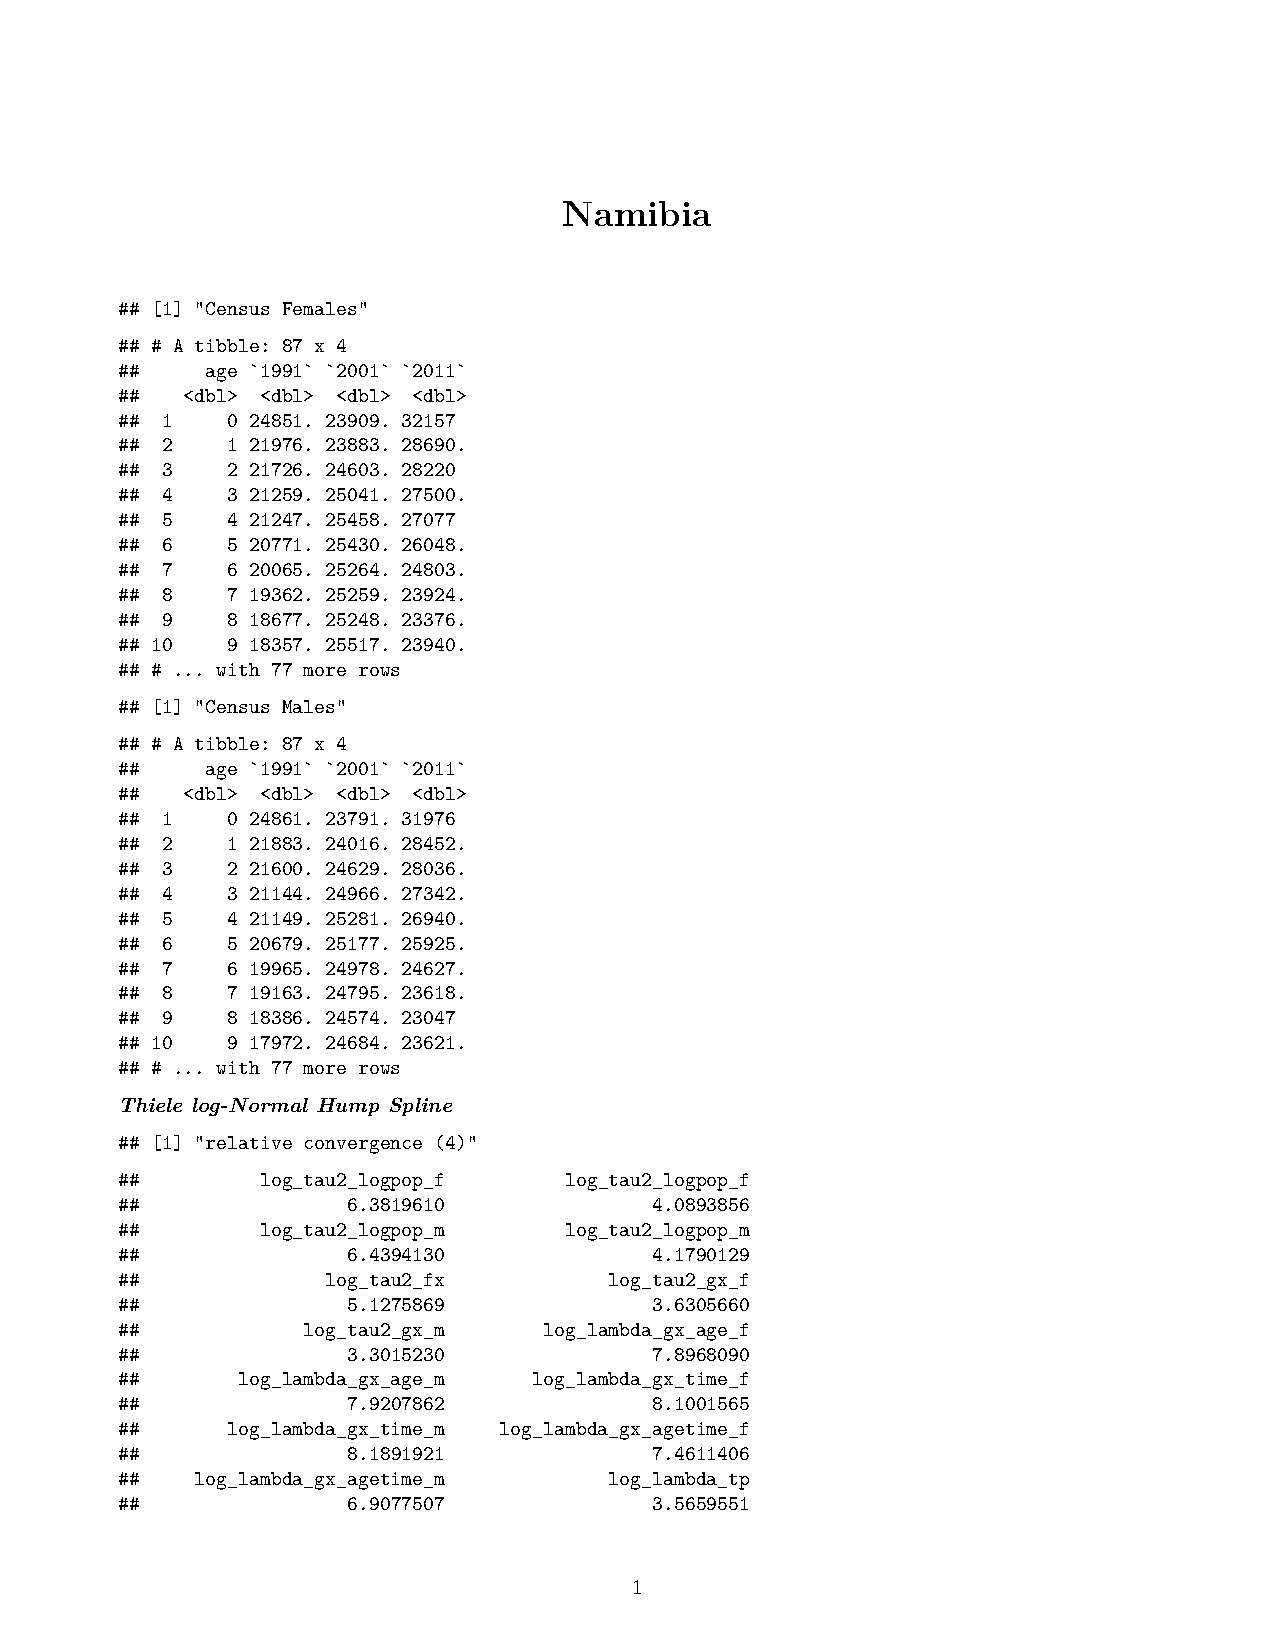
\includepdf[pages=-]{"../Rmd_RW_only_5-74_LQinit_spline/Namibia spline.pdf"}

\end{document} 